\section{\texorpdfstring{Funkce - podprogram}{Funkce - podprogram}}

% =====================================================================================================================
	\begin{frame}
    \frametitle{Funkční volání}
		
		
		\begin{itemize}
			\item Část podprogramu je volána opakovaně z různých míst programu:
			\begin{itemize}
				\item[$\Rightarrow$] musí se chovat stejně jako skoky,
			\end{itemize}
			
			\vspace{3mm}
			\item po provedení podprogramu pokračuje hlavní program z místa, kde byla funkce volána:
			\begin{itemize}
				\item[$\Rightarrow$] je nutné uchovávat návratovou hodnotu,
			\end{itemize}
			
			\vspace{3mm}
			\item může obsahovat parametry:
			
			\begin{itemize}
				\item[$\Rightarrow$] předání pomocí určených registrů (A, X, ...),
				\item[$\Rightarrow$] předání pomocí zásobníku (STACK),
			\end{itemize}
			
			\vspace{3mm}
			\item může mít návratovou hodnotu:
			\begin{itemize}
				\item[$\Rightarrow$] téměř výhradně pomocí určeného registru (A, X, ...).
			\end{itemize}
		\end{itemize}

	\end{frame}
	
% =====================================================================================================================
	\begin{frame}
    \frametitle{Instrukce CALL}
		\textbf{Příklad:} \textcolor{blue}{\textbf{CALL}} \textcolor{red}{tato\_funkce} \hspace{3mm} \textcolor{teal}{; skok na řádek tato\_funkce}
		
		\small
		
		\begin{itemize}
			\item Instrukce reprezentuje absolutní skok,
			\item \textbf{P}rogram \textbf{C}ounter (programový čítač) je nejdříve zvýšen o délku instrukce \textcolor{blue}{\textbf{CALL}} (viz dále), 
			\item do zásobníku se uloží v pořadí hodnota \textbf{PCL} a \textbf{PCH} (spodní a prostřední byte \textbf{P}rogram \textbf{C}ounter). Obdoba volání:
			
			\begin{enumerate}
				\item \textcolor{blue}{\textbf{PUSH}} PCL,
				\item \textcolor{blue}{\textbf{PUSH}} PCH,
			\end{enumerate}
			
			\begin{center}
				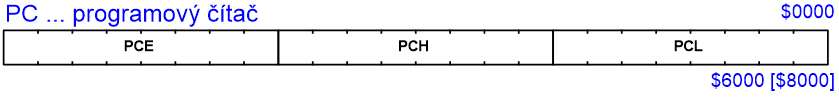
\includegraphics[width=0.9\textwidth]{fig/program_counter.png}
			\end{center}
			
			\item aktuální stav \textbf{PCH:PCL} je přepsán příslušnou adresou \uv{\textcolor{red}{tato\_funkce}},
		\end{itemize}

	\end{frame}
	
% =====================================================================================================================
	\begin{frame}
    \frametitle{Délka a trvání instrukce CALL - programovací manuál}
		
		\begin{center}
			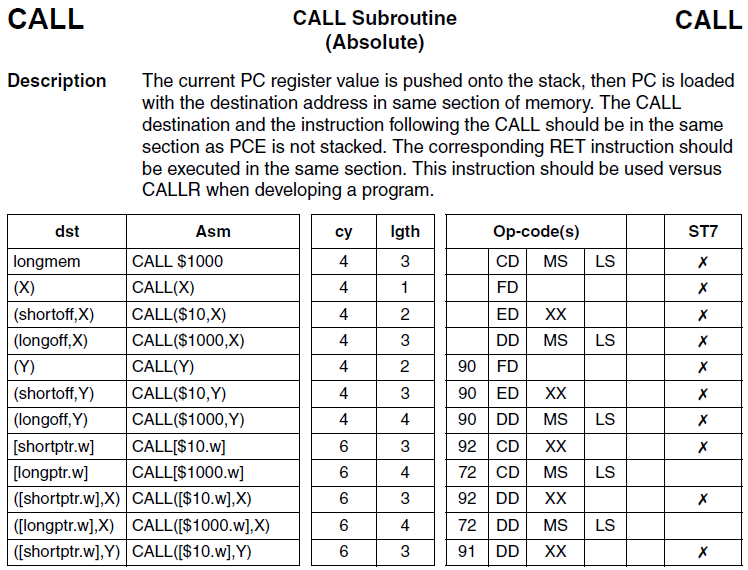
\includegraphics[width=0.80\textwidth]{fig/call.png}
		\end{center}

	\end{frame}
	
% =====================================================================================================================
	\begin{frame}
    \frametitle{Instrukce RET}
		\textbf{Příklad:} \textcolor{blue}{\textbf{RET}} \hspace{3mm} \textcolor{teal}{; skok na adresu načtenou ze zásobníku}
		
		\small
		
		\begin{itemize}
			\item Instrukce reprezentuje absolutní skok - obnovuje původní stav \textbf{PCH:PCL},
			\item ze zásobníku se získá v pořadí hodnota \textbf{PCH} a \textbf{PCL} a uloží se do \textbf{P}rogram \textbf{C}ounter. Obdoba volání:
			
			\begin{enumerate}
				\item \textcolor{blue}{\textbf{POP}} PCH,
				\item \textcolor{blue}{\textbf{POP}} PCL,
			\end{enumerate}
			
			\vspace{4mm}
			\item \textbf{PCE} se nemění, tudíž cíl skoku i návratová adresa musí být ve stejném sekci adresy \textbf{PCE},
			\item pro adresování celé paměti (delší skoky) lze použít kombinaci instrukcí \textcolor{blue}{\textbf{CALLF}} a \textcolor{blue}{\textbf{RETF}}, které upravují celou hodnotu \textbf{PCE:PCH:PCL},
			\item varianta s relativním adresováním je s instrukcí \textcolor{blue}{\textbf{CALLR}} - spoří místo v paměti (2 byte),
		\end{itemize}

	\end{frame}
	
% =====================================================================================================================
	\begin{frame}
    \frametitle{Funkce a zásobník}
		
		\small
		Návratová adresa je uložena v zásobníku:
		
		\begin{center}
			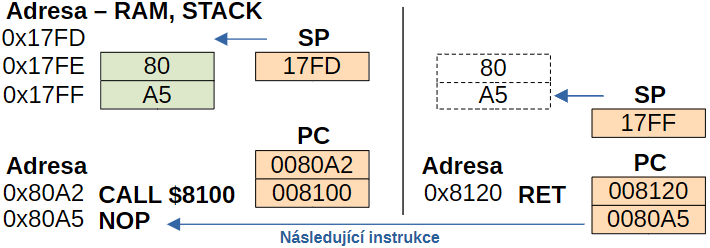
\includegraphics[width=0.90\textwidth]{fig/func-stack.png}
		\end{center}
		
		
		K datům v zásobníku lze přistupovat indexovým adresováním. Toho lze využít několika způsoby:
		
		\begin{itemize}
			\item pomocí zásobníku můžeme předávat parametry funkce,
			\item v zásobníku můžeme vytvářet lokální proměnné dané funkce,
			\item můžeme měnit návratovou adresu funkce.
		\end{itemize}

	\end{frame}
	
% =====================================================================================================================
	\begin{frame}
    \frametitle{Jazyk C, překladač pro STM8 \textbf{COSMIC}}
		
		\small
		\textbf{Volání funkce:}
		
		\begin{itemize}
			\item Název funkce v \textbf{C} je na začátku překladačem doplněn o znak \textbf{\uv{\_}} (krátká adresa - \textcolor{blue}{\textbf{CALL}}) nebo o \textbf{\uv{f\_}} (dlouhá adresa - \textcolor{blue}{\textbf{CALLF}}),
			\item pokud má funkce jeden parametr, tak je předán pomocí reistru \textbf{A} (BYTE) nebo \textbf{X} (WORD) a po skoku instrukcí \textcolor{blue}{\textbf{CALL}} je uložen do zásobníku,
			\item další parametry se ukládají do zásobníku před voláním instrukce \textcolor{blue}{\textbf{CALL}}
		\end{itemize}
		
		\vspace{4mm}
		
		\textbf{Příklad:} (char = byte)
		
		\textcolor{red}{\textbf{char}} tatoFunkce(\textcolor{red}{\textbf{char}} arg1, \textcolor{red}{\textbf{char}} arg2, \textcolor{red}{\textbf{char}} arg3)
		\begin{center}
		\textbf{STACK:}
			\begin{tabular}{| c | c | c | c | c | c |}
				\hline
				\textbf{SP} & \textbf{SP+1} & \textbf{SP+2} & \textbf{SP+3} & \textbf{SP+4} & \textbf{SP+5} \\
				\hline
				--- & arg1 & PCH & PCL & arg2 & arg3 \\
				\hline
			\end{tabular}
		\end{center}

	\end{frame}
	
% =====================================================================================================================
	\begin{frame}
    \frametitle{Jazyk C, překladač pro STM8 \textbf{COSMIC}}
		
		\small
		\textbf{Lokální proměnné}
		
		\begin{itemize}
			\item vytvářejí se zásadně v zásobníku, proměnná má platnost jen po dobu trvání funkce,
			\item funkce může volat sama sebe - \textbf{REKURZE}.
		\end{itemize}
		
		\vspace{4mm}
		
		\textbf{Příklad:} \hspace{15mm}\textcolor{red}{\textbf{char}} tatoFunkce(\textbf{void}) \{
		\begin{center}
			\begin{tabular}{l l}
				\textcolor{red}{\textbf{char}} & promenna0 = 0;\\
				\textcolor{red}{\textbf{char}} & promenna1 = 0;\\
				\textcolor{red}{\textbf{char}} & promenna1 = 0;\\
				\textcolor{blue}{\textbf{return}} & 0; \}
			\end{tabular}
		\end{center}

		\begin{center}
		\textbf{STACK:}
			\begin{tabular}{| c | c | c | c | c | c |}
				\hline
				\textbf{SP} & \textbf{SP+1} & \textbf{SP+2} & \textbf{SP+3} & \textbf{SP+4} & \textbf{SP+5} \\
				\hline
				- & promenna2 & promenna1 & promenna0 & PCH & PCL \\
				\hline
			\end{tabular}
		\end{center}

	\end{frame}
	
% =====================================================================================================================
	\begin{frame}
    \frametitle{Jazyk C, překladač pro STM8 \textbf{COSMIC}}
		
		\small
		\textbf{Návratová hodnota}
		
		\begin{itemize}
			\item u většiny překladačů (podle typu procesoru) se používá některý ze systémových registrů,
			\item registr \textbf{A} je pro návratovou hodnotu velikosti 1 BYTE nebo stejně velký ukazatel,
			\item registr \textbf{X} je pro návratovou hodnotu velikosti 1 WORD nebo stejně velký ukazatel,
			\item pro více bytové návratové hodnoty je vyhrazeno speciální paměťové místo v RAM (\textbf{c\_lreg}).
		\end{itemize}

	\end{frame}